\newpage

\chapter{Мотивация и постановка задачи}
\label{ch:chapter_1}

\section{Диаграммы связей}
\label{sec:mindmaps}
Диаграмма связей представляет собой древовидную структуру, пример на
рис.~\ref{pic:mindmap}.

\begin{figure}[h!]
  \centering
  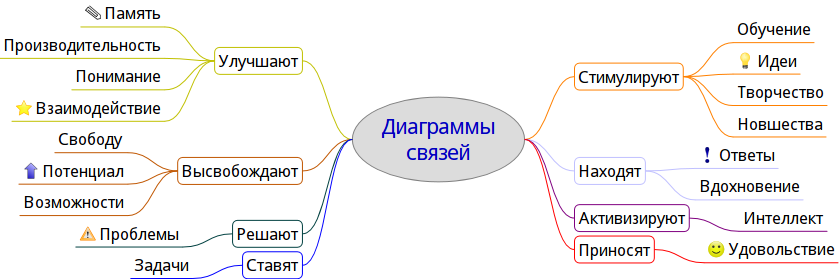
\includegraphics[width=1\linewidth]{mindmap}
  \caption{Пример диаграммы связей}
  \label{pic:mindmap}
\end{figure}

Возможность сворачивать узлы дает большее удобство для редактирования больших
диаграмм, возможность сосредоточиться на какой то отдельной части диаграммы. Так
же при различном оформлении отдельных узлов (цвет текста, цвет фона, рамка
вокруг текста, применение пиктограмм), соединительных линий можно повысить более
четкое разграничение различных частей диаграммы. Облака обычно применяются для
выделения очень важных ключевых идей. В диаграммах связей могут быть
использованы гиперссылки на веб-страницы, локальные файлы или адреса электронной
почты. Так же используются графические связи, чтобы показать взаимосвязь
элементов, находящихся в различных частях диаграммы. На рис. можно видеть пример
применения некоторых вышеописанных атрибутов узлов.


\section{Описание проекта HiveMind}
\label{sec:project_summary}
Мобильные устройства получили большое распространение в современном мире.
Зачастую, приложением, предназначенным для использования на персональном
компьютере, почти невозможно пользоваться на мобильных устройствах. Специфика
мобильных устройств, по сравнению с персональным компьютерами, заключается в
малом разрешении экрана и наличии альтернативных средств ввода. Данные различия
требуют абсолютно иного подхода к построению пользовательских интерфейсов на
мобильных устройствах. Множество людей пользуются мобильными устройствами вне
дома и персональными компьютерами у себя дома. Пользователь использует множество
операционных систем: Windows, Linux, MacOS дома и Maemo, Android, MeeGo на
мобильных устройствах. Пользователь нуждается в том, чтобы необходимое ему
приложение было доступно под все виды используемых им платформ. Данный факт
ставит перед разработчиками приложений абсолютно новую задачу  ''--- разработка
кроссплатформенных приложений с интерфейсом оптимизированным под настольные и
мобильные платформы \cite{hivemind-8th-fruct}.

Существует множество приложений для редактирования диаграмм связи (FreeMind,
Xmind, Vym, iMindMap и т.д.) и веб сервисов в сети интернет (MindMeister,
Mind42, Mindomo и т.д.). К сожалению многие из них платные, другие же,
бесплатные, имеют малую функциональность и лишь немногие имеют поддержку
совместного редактирования диаграмм связи.

Главной целью проекта HiveMind является разработка кроссплатформенного редактора
диаграмм связей, поддерживающего функции совместного редактирования.
Основные возможности:
\begin{itemize}
\item Чтение и запись файлов в формате FreeMind
\item Отображение диаграмм связей и навигация по ним
\item Интерфейс, оптимизированный для настольных и мобильных устройств
\item Интернационализация
\item Использование клавиатуры и сенсорного дисплея
\end{itemize}

Приложение HiveMind написано на языке программирования Python с использованием
библиотеки Qt для построения графического интерфейса.


\section{Совместное редактирование диаграмм связи}
\label{sec:collaborative_mindmapping}

В общем виде, процесс совместного редактирования диаграмм должен выглядеть
следующим образом. Один пользователь с установленным приложением HiveMind в
любой момент может открыть доступ к своей диаграмме связи. Другой пользователь
подключается к диаграмме связи данного человека и автоматически получает её
актуальную копию, после чего оба пользователя начинают совместное
редактирование. Для того чтобы предоставить различные сценарии
совместного взаимодействие, на сервере должна быть возможность изменять права
участников и режимы доступа карте. Далее будут перечислены возможные сценарии
совместного взаимодействия.

Пользователь создаёт диаграмму связи и начинает её редактирование, используя
мобильное устройство, ноутбук или персональный компьютер. В процессе
редактирования пользователь решает показать свою работу другу (к примеру, для
получения помощи). Для того чтобы сделать данное действие возможным, он
открывает доступ к своей диаграмме. В данном случае ноутбук или мобильное
устройство пользователя работает как сервис, доступный из локальной сети или
интернет. Другой пользователь подключается к диаграмме связи и автоматически
получает актуальную версию диаграммы. Далее оба пользователя начинают совместное
редактирование диаграммы. Количество взаимодействующих участников неограниченно,
поэтому другие пользователи также могут участвовать в совместной работе.
Изменения, совершаемые каждым из участников, незамедлительно посылаются
остальным участникам.

Следующий сценарий использования совместного редактирования диаграмм связи может
быть полезен при представлении докладов. К примеру, докладчик имеет
дополнительные материалы, такие как: план презентации, краткий обзор речи
выстпуление или ссылки на дополнительные ресурсы. Докладчик оформляет данные
материалы в виде диаграммы связи и открывает к ней доступ. Используя HiveMind
cлушатели подключаются к диаграмме связи, выложенной докладчиком, используя свои
мобильные устройства или нетбуки. Таким образом слушатели получают материалы
подготовленные докладчиком, а также все изменения, сделанные докладчиком в
процессе выстпуления и позволяющие более ясно предоставить материал доклада.

Диаграмма связи также может содержать материалы для дискуссии в реальном
времени. В данном случае она может быть использована как лекционная доска с
иерархической структурой, на которую каждый участник может заносить свои идеи,
комментарии или мнения. Главное преимущество такого рода обсуждений с
исполльзованием HiveMind то, что все данные имеют иерархическую структуру и
доставляются всем участникам почти мгновенно.

Пользователь может хранит на диаграмме связи свою личную информацию, поэтому,
открывая доступ к диаграмме связи, он должен иметь возможность ограничить
возможность присоединения к диаграмме только избранному кругу лиц. Также он
должен иметь возможность контролировать права доступа участников на
редактирование. К примеру, при выступлении двух докладчиков перед аудиторией,
необходимо разрешить редактирование диаграммы только выстпуающим и
запретить всем остальным.


\section{Постановка задачи}
\label{sec:problem_statement}
